\chapter{OpenSHMEM在Tilera平台上的实现框架}
\section{Tilera Gx8036平台简介}

Tilera公司是位于硅谷的新创无晶圆半导体公司,因为在多核技术方面拥有独家的先进技术,该公司曾被美国知名媒体EETIMES评为全球最有希望的60家新兴企业之一。
2009年11月,Tilera公司发布了令其公司名声大震的众核平台GX系列,其中包括拥有100个核心的TILE-Gx100,同时也有本文用于搭建OpenSHMEM简单框架的Gx8036平台。Tile-Gx系列采用40nm处理器制造工艺,CPU时钟频率为1.2GHz。Tile-Gx系列尤其注重对功耗的把握,在运行一个典型的网络应用的情景下,该平台的运行功耗约为25~30W,考虑到该平台极高的集成度,这个功耗值约为同等高性能处理器的1/2到1/4。
在这个平台上,36个通用核中的每一个都是相同的64位处理器,每个处理器都带有私有本地缓存,并且实现了一个较为复杂的虚拟内存系统。每个核上都可以单独的跑一个自己的操作系统,也可以多个核成组运行一个SMP操作系统,本文的实现环境就是Tielra提供的SMP Linux。

\begin{figure}
\centering
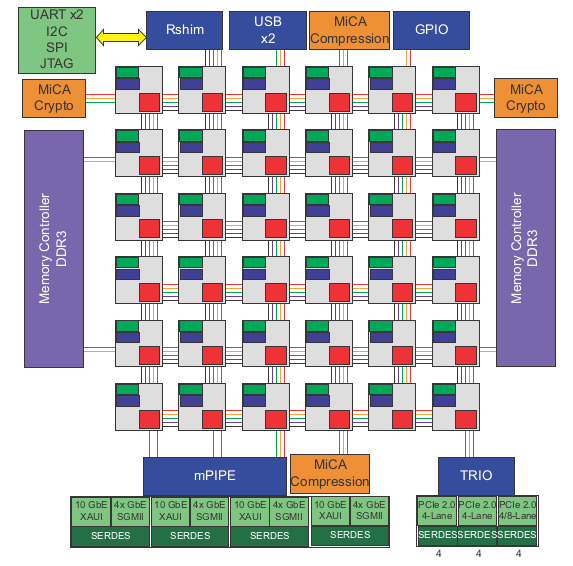
\includegraphics[scale=0.5]{Tile36_Block_Diagram.png}
\caption{TILE-Gx36平台示意图}\label{fig:TILEs-DIA}
\end{figure}

TILE-Gx36的硬件架构如 图~\ref{fig:TILEs-DIA} 所示。由图中可以看出,TILE-Gx36平台提供了相当丰富的外设接口资源,尤其针对对于网络流的处理做了硬件优化。但是在本次实现中,暂时不考虑通过外部网络级联两个或以上板卡扩展性能的情况,仅在一个平台内进行实验。TILE-Gx36平台中每个核是通过片上高速网络iMesh相连接。根据\cite{jour:NoC}关于高速片上网络拓扑结构的比较,Mesh或者Mesh-like网络结构是现有可靠的、高速的、低功耗的片上网络结构的主要实现,并且呈现越来越广泛的使用趋势。在TILE-Gx36平台上,使用的是Tilera公司的iMesh技术。iMesh是基于Mesh网络结构的高速片上互联网络的高带宽、低延迟的实现。iMesh网络互联的tile可以通过网络快速的访问其他tile的缓存、外部主存以及I/O。 并且,在TILE-Gx36上实现的分布式共享一致性缓存架构,解决了网络访问的瓶颈问题,并且最小化了功耗。在TILE-Gx8036中,提供了如图~\ref{fig:TILE-network}的5个动态网络(Dynamic Network, DN),分别连接相邻的两个tile,提供快速的数据、指令交换策略。这5个网络连接中,对于用户层可用的为UDN(User Dynamic Network)以及IDN(Instruct Dynamic Network),由于UDN的表现以及性能对于OpenSHMEM的实现比较重要,将在下文以及平台测试部分再次详细讨论。\\
\begin{figure}
\centering
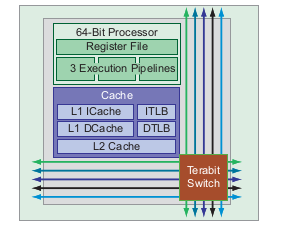
\includegraphics{Tile_Detail.png}
\caption{TILE-Gx36中Tile结构以及片上网络示意图}\label{fig:TILE-network}
\end{figure}

另一方面,在前面的讨论中可知,影响多核平台编程以及性能表现的另外一个因素即为内存子系统。在TILE-Gx36平台中,每个处理单元拥有私有的片上cache系统以及memory controller, 但是需要和其他tile共享一个内存系统。这样的内存系统结构可以同时提供对共享内存模型以及消息传递模型的较好的硬件支持。
\subsection{Tile-Gx36平台的片上网络}
\subsection{Tile-Gx36平台的内存体系}

\section{平台性能测试设计}
\subsection{Common Memory的性能测试}
\subsection{Spin与Barrier同步原语的延迟性能测试}
\subsection{UDN用户空间中断性能测试}
\subsection{UDN性能测试}

\section{OpenSHMEM实现设计}
\subsection{环境建立}
\subsection{put与get}
\subsection{集体操作}